%programming realization

\textcolor{red}{
TODO: здесь должно быть объяснение, почему мы включаем именно в Фумили.
Ну, или он должно появиться в предыдущей части, где мы рассказывали про Фумили.
}

%очень общая схема включения дополнения в Fumili и ROOT
% \centering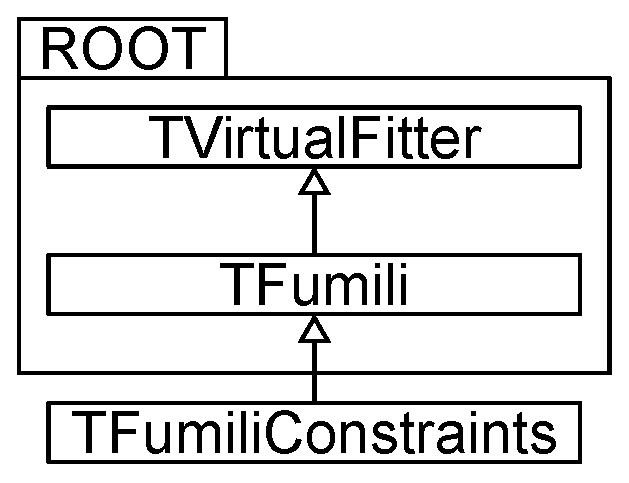
\includegraphics[width=0.4\textwidth]{pics/arch1.eps}

% \begin{figure}[htbp]
% \centering
% \centering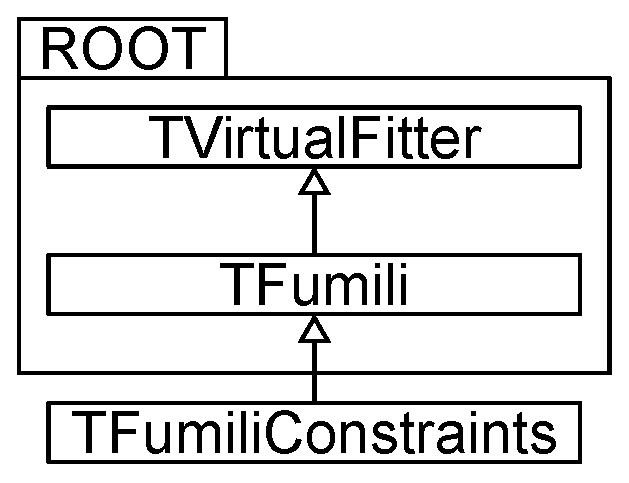
\includegraphics[width=0.35\textwidth]{pics/arch1.eps}
% \caption{
% Схема отношений классов при фитировании.
% Разработанный авторами класс TFumiliConstraints наследует от класса TFumili.
% }
% \label{arch}
% \end{figure}

%фактический user API. Несколько избыточен для статьи и вообще недоработан
% \begin{verbatim}
% void FCN(int & n_par, double * grad,
%          double & val, double * par, int flag);
% /* ... */
% TFumiliConstraints * fum = new TFumiliConstraints;
% // set parameters
% fum->SetParNumber(2);
% fum->SetParameter(0, "#alpha", .5, 0.01, 0, 0);
% fum->SetParameter(1, "#beta", .0, 0.01, 0, 0);
% // set constraints
% fum->SetConstrNumber(1);
% fum->SetConstraint(0, [](double * p){
%   return p[0]*p[0] + .5*p[1] - 1.3;
% });
% fum->SetConstrDeriv(0, 0, [](double * p){ return 2*p[0]; });
% fum->SetConstrDeriv(0, 1, .5);
% // set objective function
% fum->SetFCN(FCN);
% // minimize
% fum->Minimize();
%
% \end{verbatim}

